\documentclass[11pt]{article}

\usepackage[a4paper]{geometry}
\geometry{left=2.0cm,right=2.0cm,top=3cm,bottom=2.5cm}
\usepackage{setspace}
\setstretch{1.5}
\usepackage{ctex}
\usepackage{amsmath,amsfonts,graphicx,amssymb,bm,amsthm}
\usepackage{algorithm,algorithmicx}
\usepackage[noend]{algpseudocode}
\usepackage{fancyhdr}
\usepackage{booktabs}
\usepackage{array}
\usepackage{float}
\usepackage{listings}
\usepackage{xcolor}

\lstset{
	language=Python,
	basicstyle=\ttfamily\small,
	numbers=left,
	numberstyle=\tiny\color{teal!70!black},
	showstringspaces=false,
	breaklines=true,
	frame=single,
	rulecolor=\color{black},
	framerule=0.6pt,
	framesep=4pt,
	xleftmargin=6pt,
	backgroundcolor=\color{gray!4},
	columns=fullflexible,
	keywordstyle=\bfseries\color{blue!70!black},
	commentstyle=\itshape\color{green!50!black},
	stringstyle=\color{red!60!black},
	identifierstyle=\color{violet!70!black},
	emphstyle=\bfseries\color{orange!80!black},
	tabsize=4
}
\newcolumntype{M}[1]{>{\centering\arraybackslash}m{#1}}
\setlength{\headheight}{14pt}

\begin{document}
	\pagestyle{fancy}
	\lhead{\kaishu 中国科学院大学}
	\chead{}
	\rhead{\kaishu 2026年春季学期\qquad 深度学习}
	
	\begin{center}
		{\LARGE \bf 实验二：基于ViT的CIFAR10图像分类}
	\end{center}
	\begin{center}
		\large\kaishu{尧祥临 202518023406038 前沿交叉科学学院}
	\end{center}

	\section{任务介绍}
	本次实验的任务是基于Vision Transformer（ViT）模型完成CIFAR10图像分类。实验指导书要求从零开始完成数据读取、网络构建、模型训练和模型测试等过程，并在CIFAR10数据集的测试集上达到80\%以上的分类准确率。

	CIFAR10数据集包含60000张$32\times 32$彩色图像，共10个类别，分别为airplane、automobile、bird、cat、deer、dog、frog、horse、ship和truck。官方训练集包含50000张图像，测试集包含10000张图像。本实验将官方训练集划分为45000张训练样本和5000张验证样本，官方测试集保持为10000张，用于最终评估。

	\section{模型架构}
	本实验实现的是适配CIFAR10小尺寸图像的ViT模型。由于CIFAR10图像尺寸为$32\times 32$，这里没有将图像放大到标准ViT常用的$224\times 224$，而是直接在原始分辨率上进行patch划分。模型整体由Patch Embedding、位置编码、Transformer Encoder和分类头组成。

	\subsection{Patch Embedding}
	输入图像大小为$3\times 32\times 32$，patch大小设置为$4\times 4$，因此每张图像会被划分为
	\[
		N=\left(\frac{32}{4}\right)^2=64
	\]
	个patch。代码中使用一个卷积层完成patch划分和线性投影，其卷积核大小和步长都等于patch大小，因此卷积输出为$256\times 8\times 8$，展平并转置后得到$64\times 256$的token序列。

	\begin{lstlisting}
class Embedding(nn.Module):
    def __init__(self, image_size=32, patch_size=4,
                 in_channels=3, embed_dim=256):
        super().__init__()
        self.num_patches = (image_size // patch_size) ** 2
        self.embedding = nn.Sequential(
            nn.Conv2d(in_channels, embed_dim,
                      kernel_size=patch_size,
                      stride=patch_size,
                      bias=False),
            nn.Flatten(2)
        )

    def forward(self, x):
        output = self.embedding(x)
        output = output.transpose(1, 2)
        return output
	\end{lstlisting}

	\subsection{Transformer Encoder}
	每个Transformer层由多头自注意力模块、MLP模块、LayerNorm、残差连接和DropPath组成。注意力模块使用PyTorch中的\texttt{nn.MultiheadAttention}实现，并设置\texttt{batch\_first=True}，使输入维度保持为$B\times N\times D$。MLP模块由两层全连接层、GELU激活函数和Dropout组成，隐藏层维度为1024。

	\[
		\mathrm{Attention}(Q,K,V)=\mathrm{softmax}\left(\frac{QK^\top}{\sqrt{d_k}}\right)V.
	\]
	在本模型中，嵌入维度$D=256$，注意力头数为8，因此每个head的维度为32。Transformer深度设置为8，即堆叠8个编码器层。

	\begin{lstlisting}
class Transformer(nn.Module):
    def __init__(self, embed_dim=256, num_heads=8,
                 mlp_hidden_dim=1024, depth=8,
                 dropout=0.1, drop_path_rate=0.1):
        super().__init__()
        drop_path_rates = torch.linspace(0, drop_path_rate, depth).tolist()
        self.layers = nn.ModuleList([
            nn.ModuleList([
                Attention(embed_dim, num_heads, dropout),
                Mlp(embed_dim, mlp_hidden_dim, dropout),
                DropPath(drop_path_rates[layer_idx]),
                DropPath(drop_path_rates[layer_idx]),
            ])
            for layer_idx in range(depth)
        ])

    def forward(self, x):
        for attn, mlp, attn_drop_path, mlp_drop_path in self.layers:
            x = x + attn_drop_path(attn(x))
            x = x + mlp_drop_path(mlp(x))
        return x
	\end{lstlisting}

	\subsection{整体结构}
	Patch token前会拼接一个可学习的\texttt{cls\_token}，并加入可学习的位置编码。Transformer输出后，代码没有直接使用\texttt{cls\_token}做分类，而是对所有patch token取均值作为图像表示，再通过线性分类头输出10类logits。

	\begin{table}[H]
		\centering
		\caption{ViT模型主要结构}
		\begin{tabular}{M{3.8cm} M{4.2cm} M{5.5cm}}
			\toprule
			模块 & 输出形状 & 设置 \\
			\midrule
			Input & $3\times 32\times 32$ & CIFAR10彩色图像 \\
			Patch Embedding & $64\times 256$ & patch size = 4, embed dim = 256 \\
			Token + Position & $65\times 256$ & 拼接\texttt{cls\_token}并加入位置编码 \\
			Transformer Encoder & $65\times 256$ & depth = 8, heads = 8 \\
			Mean Pooling & $256$ & 对patch token求均值 \\
			Classification Head & $10$ & 输出10类logits \\
			\bottomrule
		\end{tabular}
	\end{table}

	本模型总参数量为6350346，其中Transformer Encoder约6318080个参数，是主要的参数来源。Patch Embedding参数量为12288，分类头参数量为2570。

	\section{参数设置与训练方法}
	训练阶段采用AdamW优化器，并对不同参数组设置不同的权重衰减策略：对卷积和全连接权重使用weight decay，对bias、LayerNorm参数、\texttt{cls\_token}和位置编码不使用weight decay。这样做的原因是，归一化参数和位置相关参数本身并不直接承担普通线性权重的特征压缩作用，如果对它们施加同样的衰减，可能削弱位置编码和归一化层的表达能力。

	相比卷积网络，ViT缺少卷积结构中天然的局部平移归纳偏置，在CIFAR10这种小规模数据集上更容易出现过拟合。因此训练中加入了较强的数据增强和正则化策略：随机裁剪和随机水平翻转用于扩大输入扰动，Random Erasing模拟局部遮挡，Mixup和label smoothing降低模型对单个样本标签的过度自信，DropPath约束深层Transformer的共适应。模型评估时使用EMA参数，可以降低单次梯度更新带来的参数震荡，使验证和测试指标更平稳。

	学习率策略采用前10个epoch线性warmup，随后进行余弦退火。warmup阶段让Transformer在训练初期以较小步长进入稳定区域，避免注意力权重和MLP权重在随机初始化后被过大的学习率破坏；余弦退火则在中后期逐步减小学习率，使模型从快速拟合转向细粒度收敛。

	\begin{table}[H]
		\centering
		\caption{主要训练配置}
		\small
		\begin{tabular}{M{3cm} M{3cm} M{3cm} M{3cm}}
			\toprule
			项目 & 设置 & 项目 & 设置 \\
			\midrule
			Batch size & 128 & Optimizer & AdamW \\
			初始学习率 & $4\times10^{-4}$ & Weight decay & $2\times10^{-2}$ \\
			Epochs & 200 & Early stopping & patience 40 \\
			Label smoothing & 0.05 & Mixup alpha & 0.2 \\
			Drop path & 0.1 & EMA decay & 0.9998 \\
			Gradient clip & 1.0 & Seed & 114514 \\
			\bottomrule
		\end{tabular}
	\end{table}

	\section{训练过程与实验结果}
	训练日志共记录176个epoch。验证集准确率在第136个epoch达到最高值85.68\%，之后连续40个epoch没有进一步提升，因此训练过程触发early stopping并在第176个epoch停止。日志中测试集准确率最高为85.79\%，出现在第131个epoch；验证集最优模型对应的测试集准确率为85.61\%；最后一轮测试集准确率为85.57\%。这些结果均明显高于实验指导书中80\%的要求。

	\begin{table}[H]
		\centering
		\caption{关键训练节点}
		\small
		\begin{tabular}{M{2.2cm} M{2.6cm} M{2.6cm} M{4.4cm}}
			\toprule
			Epoch & Val Acc & Test Acc & 说明 \\
			\midrule
			50  & 79.58\% & 80.59\% & 首次达到实验要求附近 \\
			100 & 84.58\% & 85.12\% & 模型进入稳定提升阶段 \\
			131 & 85.46\% & \textbf{85.79\%} & 测试集准确率最高 \\
			136 & \textbf{85.68\%} & 85.61\% & 验证集准确率最高 \\
			176 & 85.32\% & 85.57\% & early stopping停止训练 \\
			\bottomrule
		\end{tabular}
	\end{table}

	\begin{figure}[H]
		\centering
		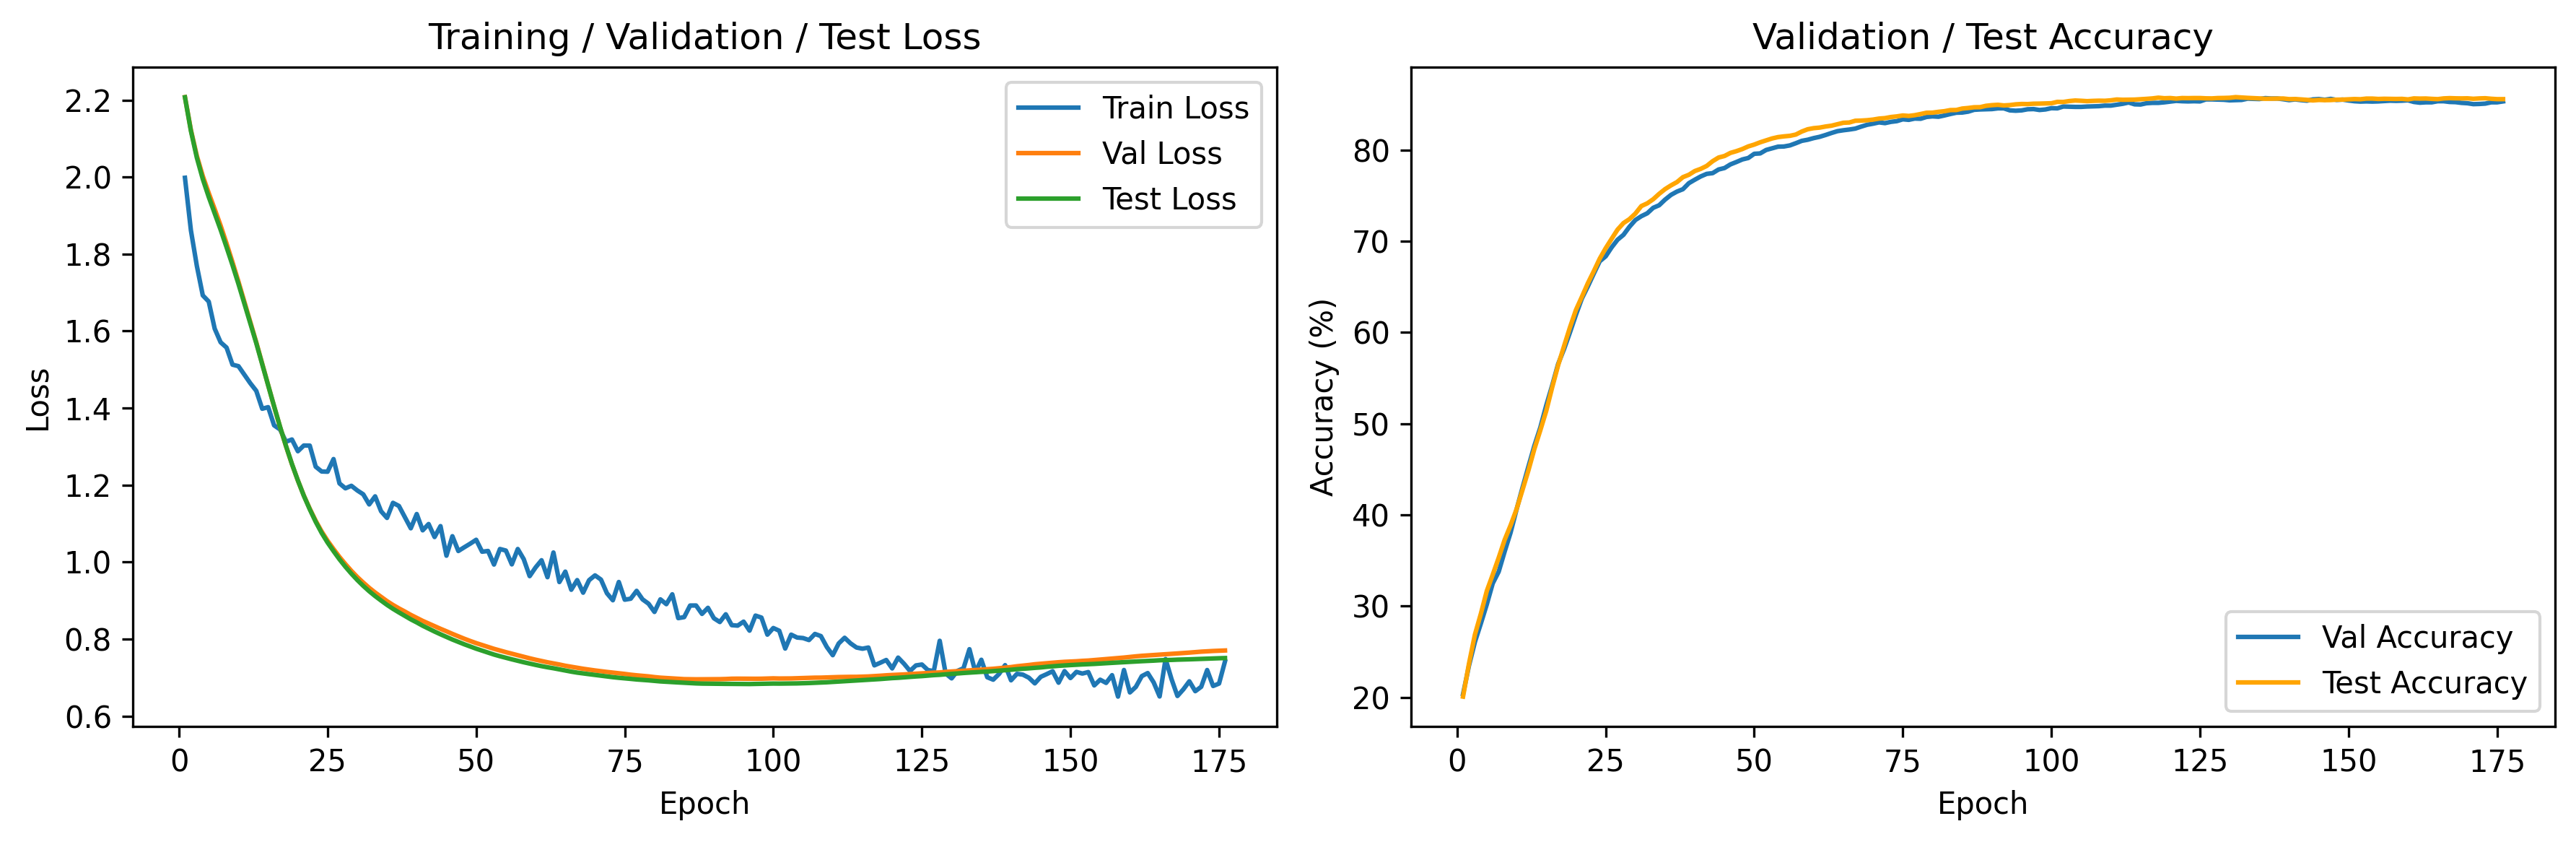
\includegraphics[width=0.96\linewidth]{../Figure/loss_acc_curves.png}
		\caption{训练损失与准确率变化曲线}
	\end{figure}

	从图1可以看到，训练前期loss下降较快，验证集和测试集准确率也快速提升。第50个epoch附近测试准确率已经达到80.59\%，超过实验要求；之后准确率继续缓慢提升，并在训练后期稳定在85\%附近。这说明模型在前半段主要完成基础特征学习，后半段则更多是在正则化和学习率衰减的共同作用下进行小幅精修。

	训练loss在后期仍有波动，但验证集和测试集曲线整体较平稳。这里的训练loss不能简单地与验证loss直接比较，因为训练阶段启用了Mixup、Random Erasing和随机裁剪，输入样本和标签都被扰动；验证和测试阶段则使用原始标签和确定性预处理。因此训练loss的波动更像是增强策略带来的优化噪声，而不是模型失效的信号。相反，验证集和测试集准确率在后期保持接近，说明模型没有出现明显的训练集记忆化问题。

	\begin{figure}[H]
		\centering
		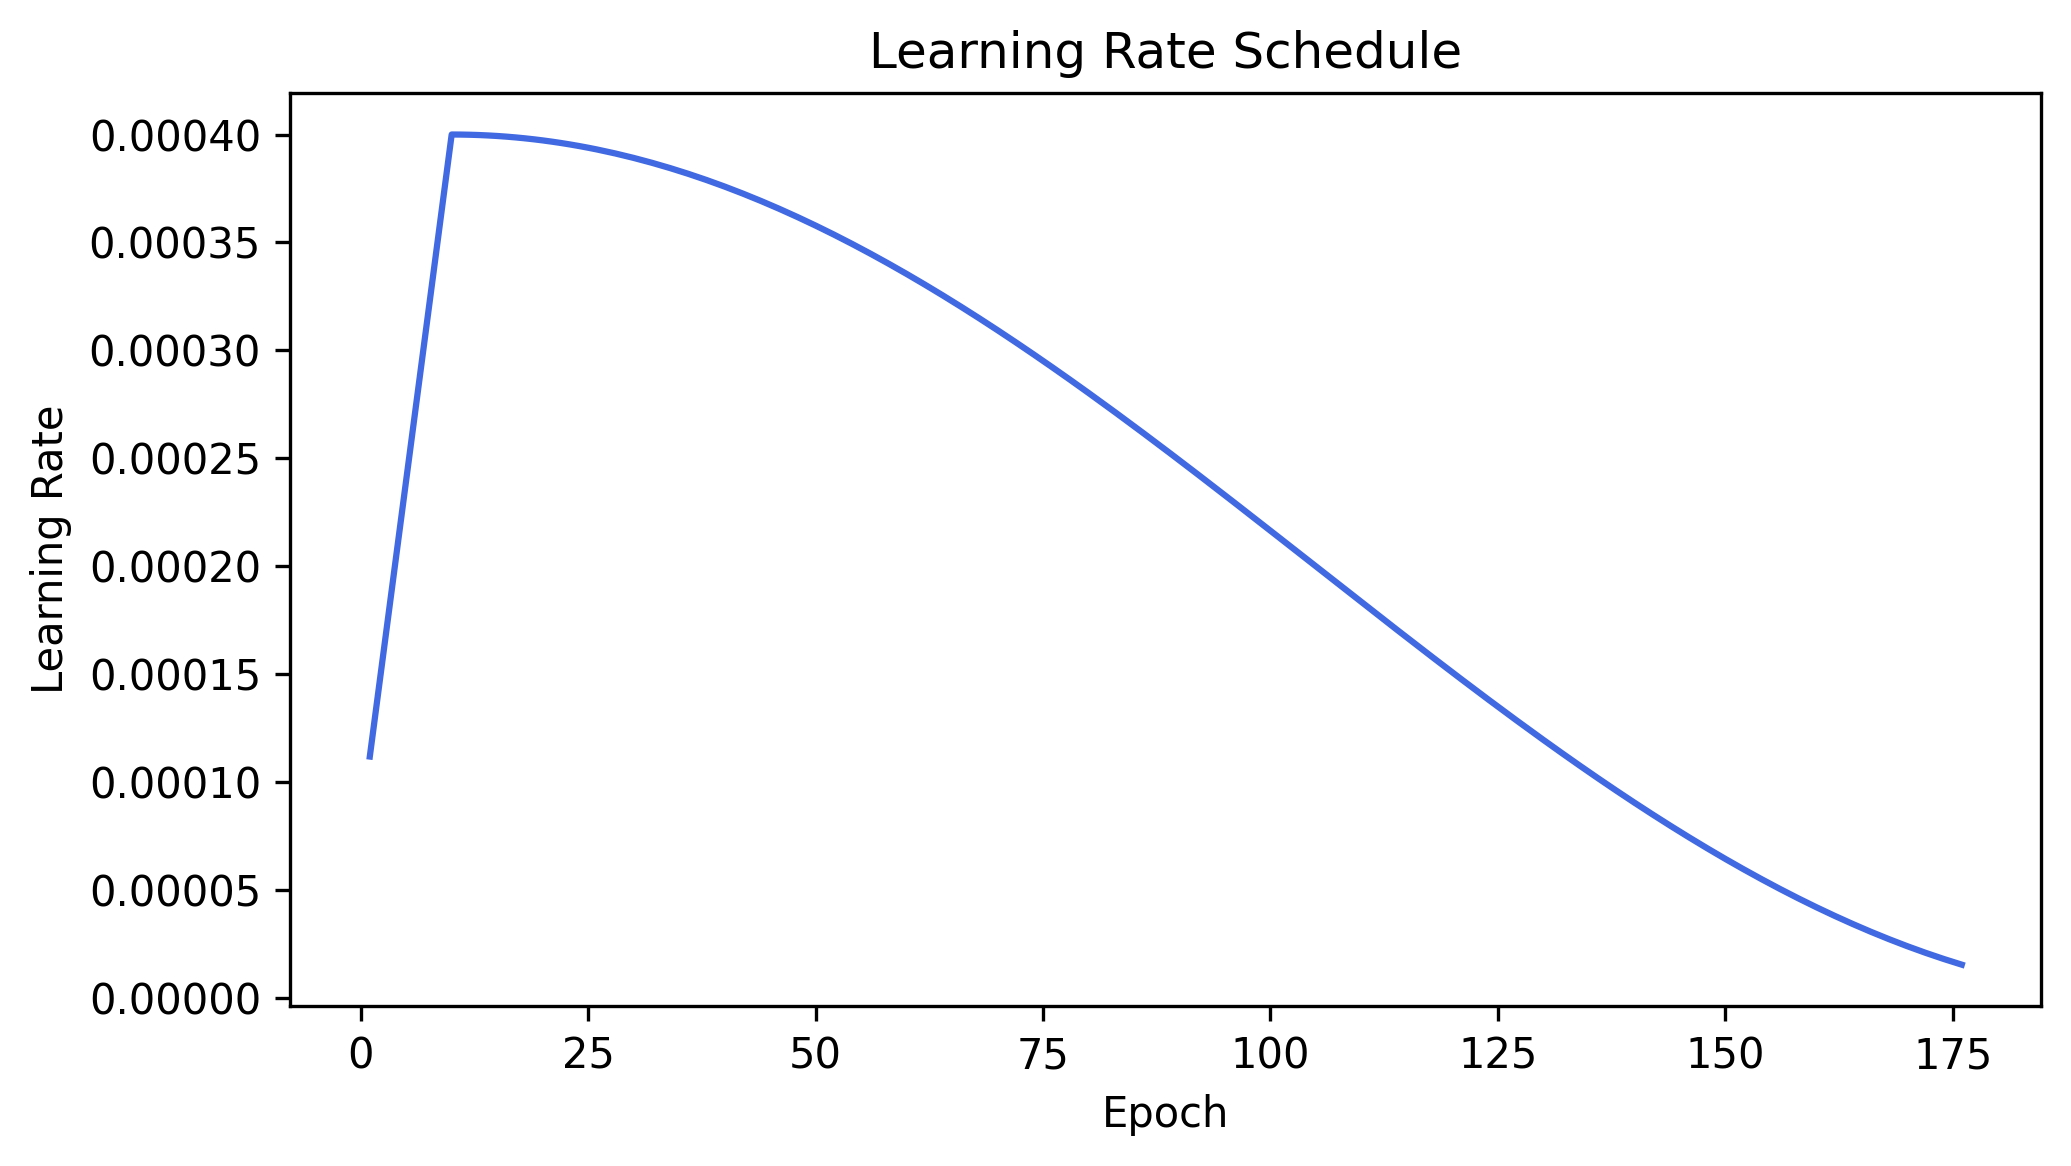
\includegraphics[width=0.68\linewidth]{../Figure/lr_curve.png}
		\caption{学习率变化曲线}
	\end{figure}

	图2展示了学习率调度过程。前10个epoch为线性warmup，学习率从较小值逐步增加到$4\times10^{-4}$；随后进入余弦退火阶段，学习率逐渐下降。该策略可以在训练早期避免模型参数剧烈震荡，并在训练后期帮助模型更稳定地收敛。

	\begin{figure}[H]
		\centering
		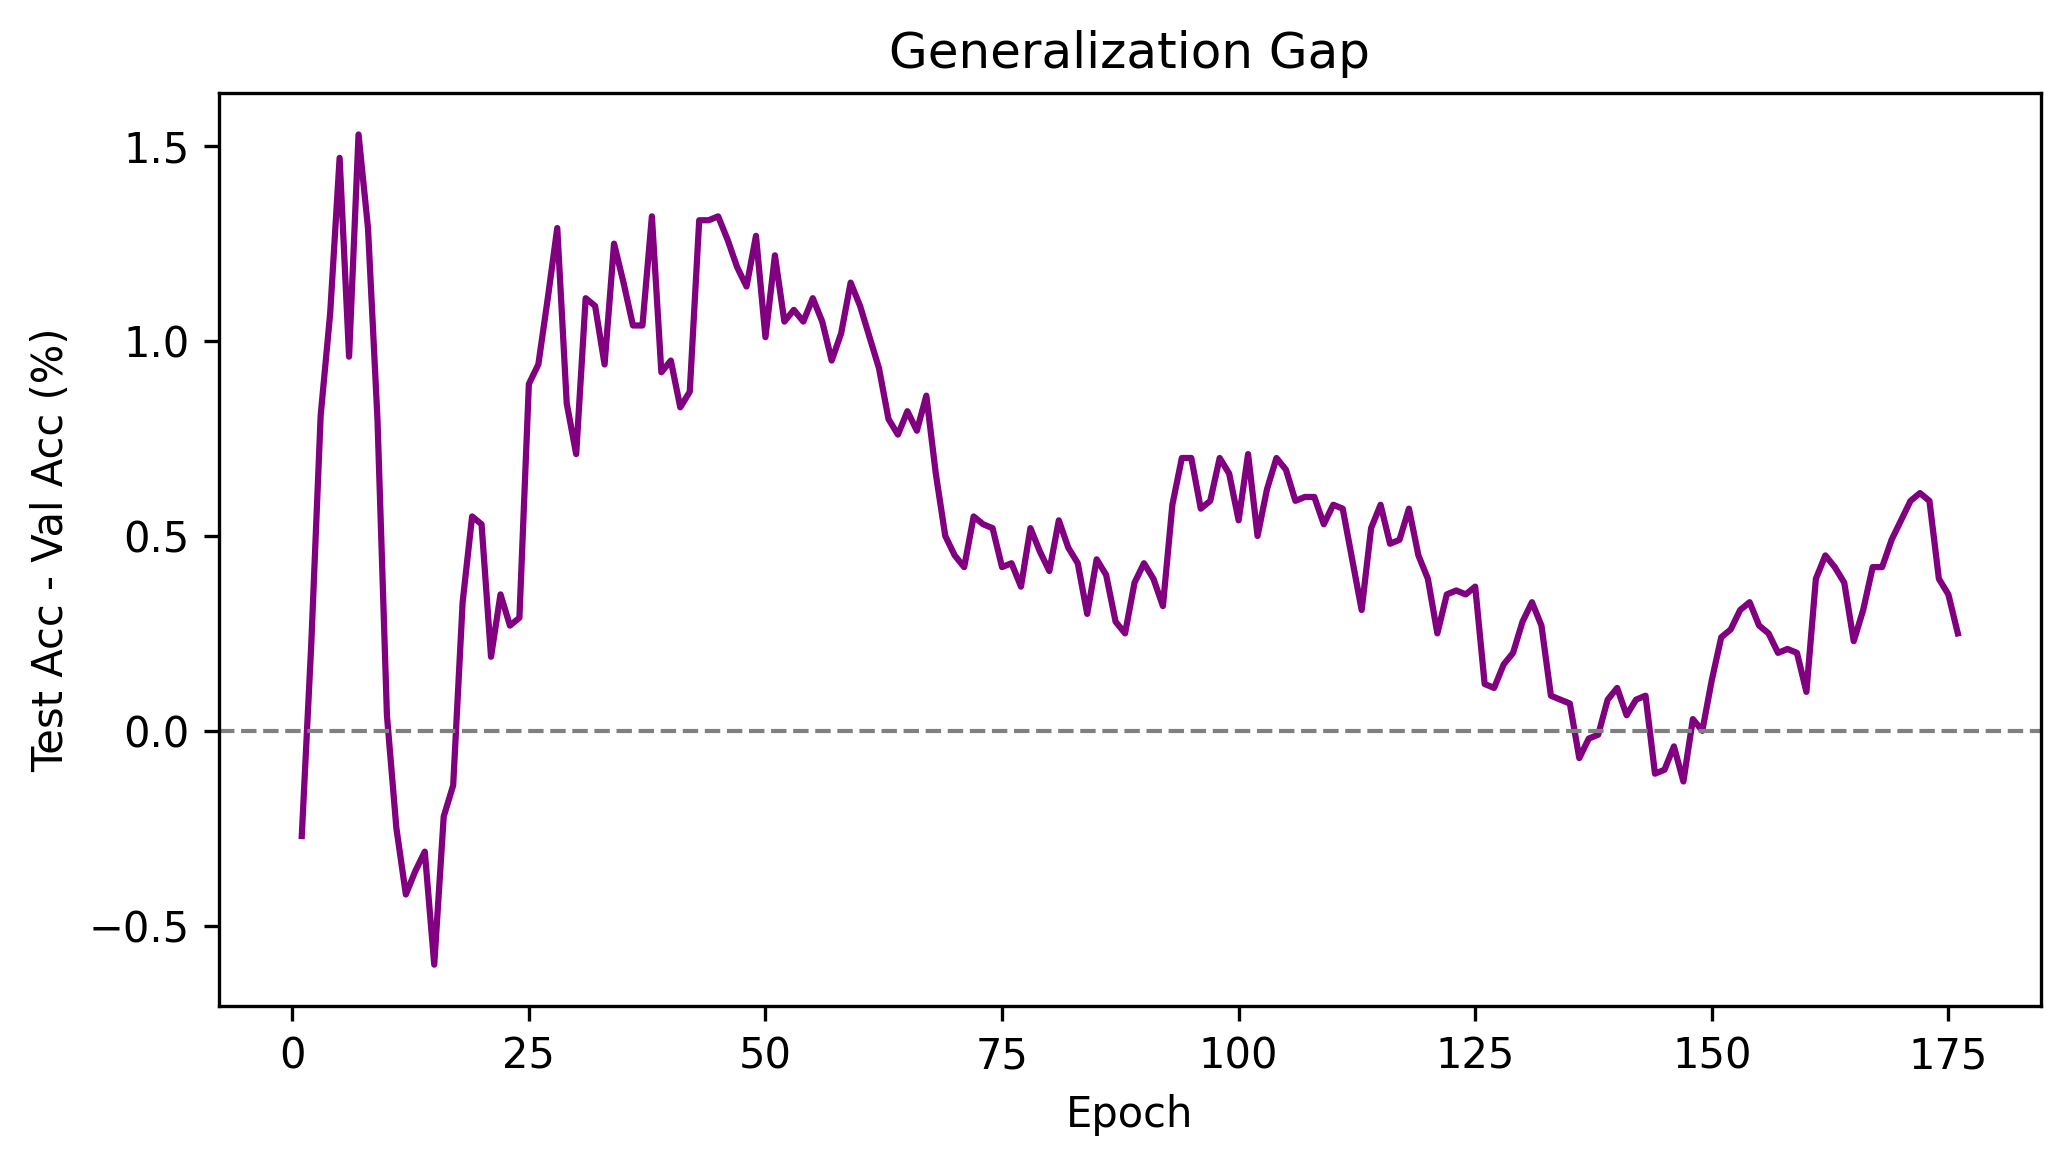
\includegraphics[width=0.68\linewidth]{../Figure/generalization_gap.png}
		\caption{测试集与验证集准确率差距}
	\end{figure}

	图3给出了测试集准确率与验证集准确率的差值。多数epoch中该差值都保持在较小范围内，说明验证集能够较好反映测试集趋势，没有出现验证集选择与测试集表现严重不一致的情况。第131个epoch测试集达到最高值，而第136个epoch验证集达到最高值，两者相差只有5个epoch；对应测试准确率分别为85.79\%和85.61\%，差距也很小。因此使用验证集最优模型作为最终提交模型是合理的。

	\begin{figure}[H]
		\centering
		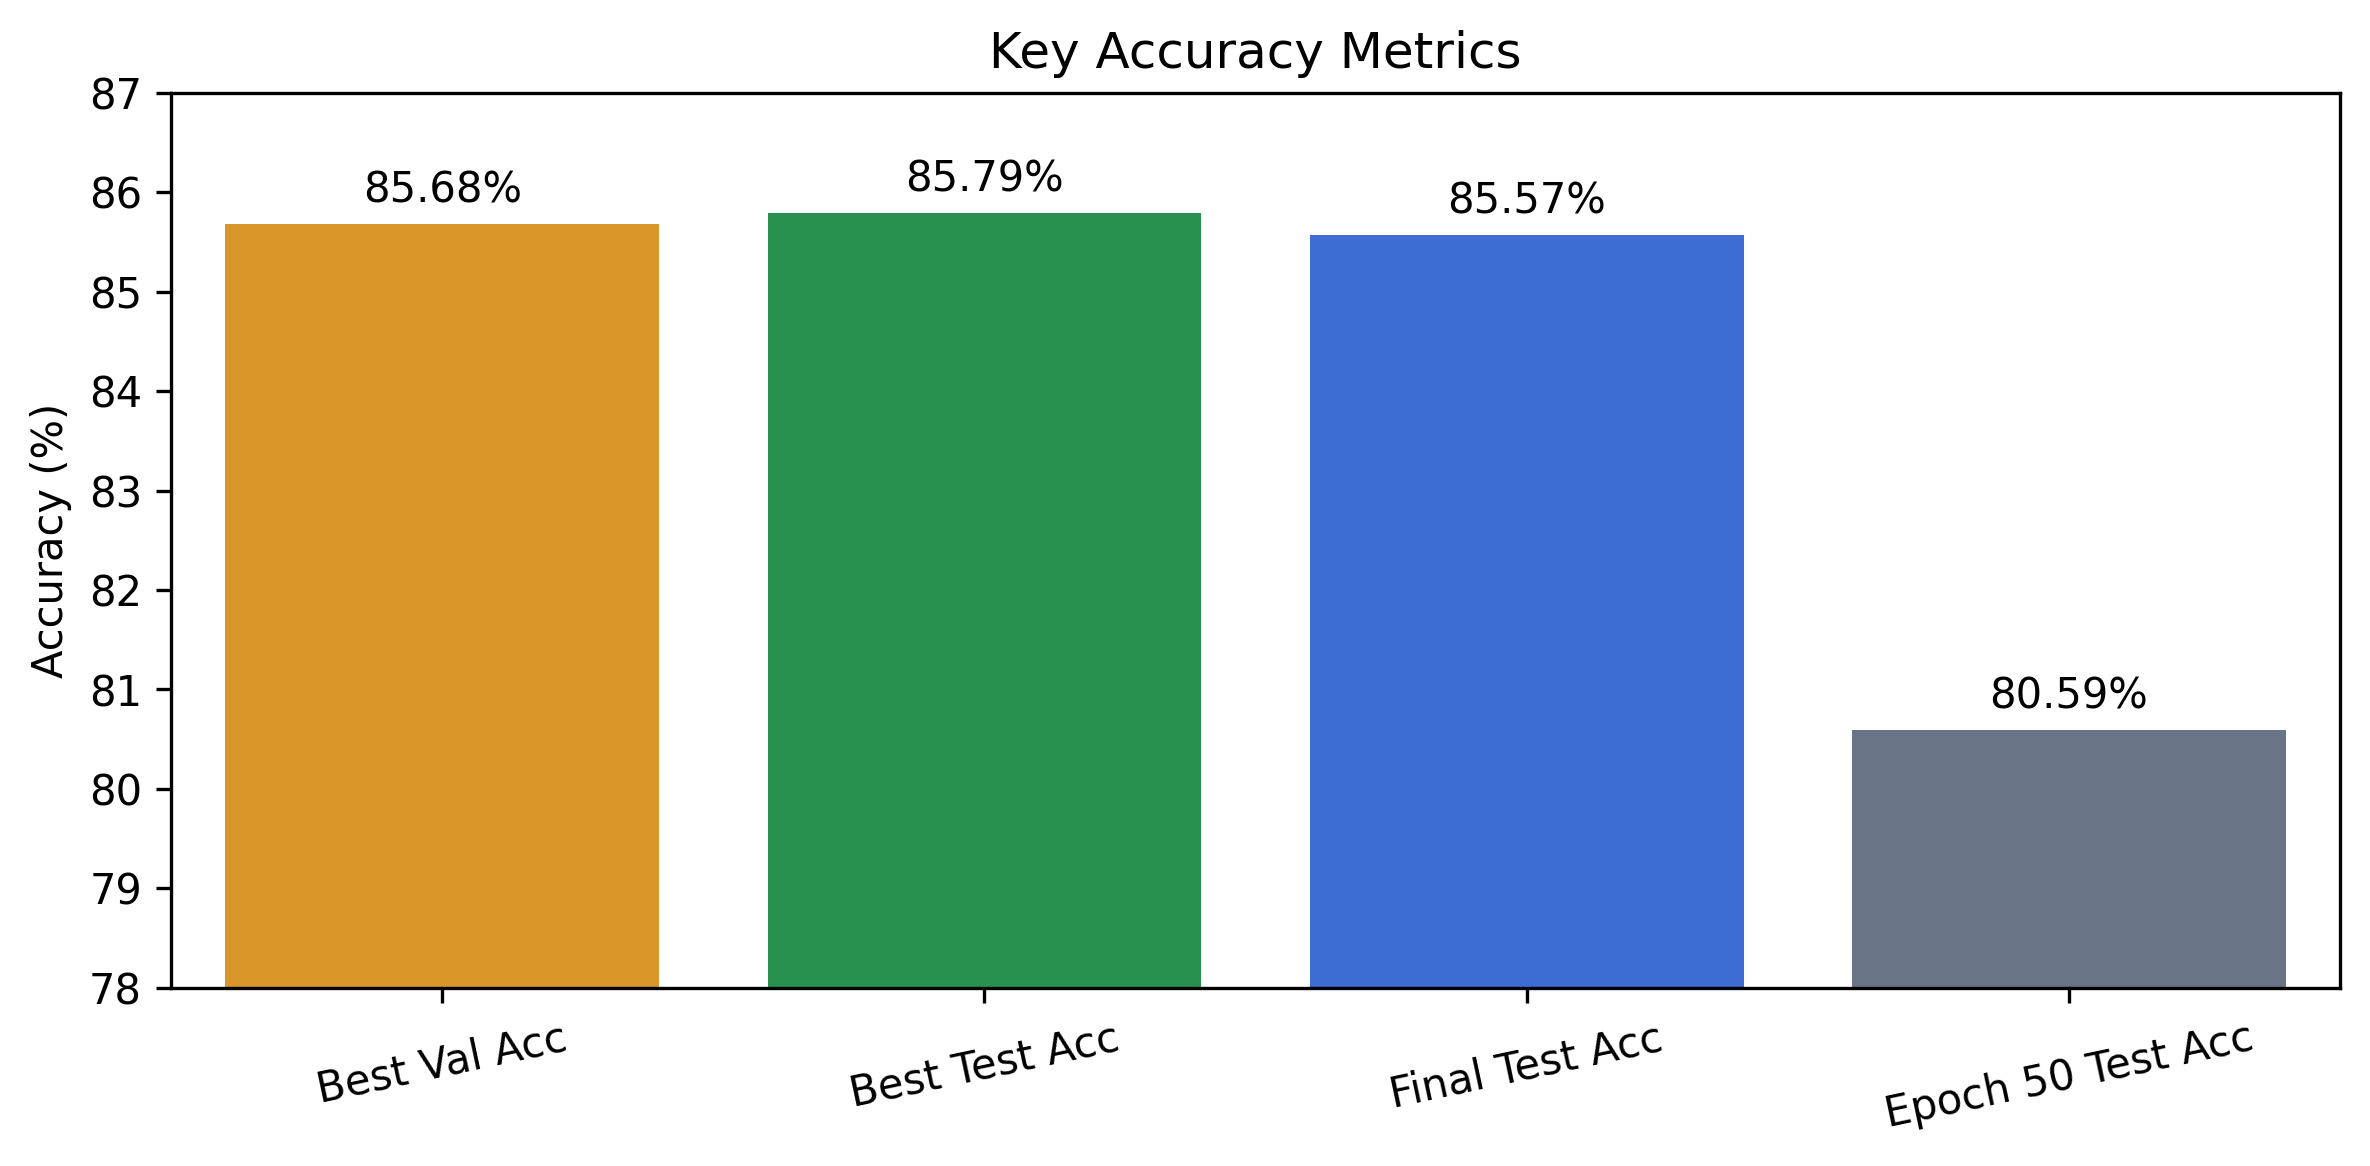
\includegraphics[width=0.68\linewidth]{../Figure/key_metrics.png}
		\caption{关键结果汇总}
	\end{figure}

	图4进一步汇总了若干关键准确率。可以看到，模型在达到80\%之后仍有约5个百分点的提升空间，但后期提升速度明显变慢。这符合ViT在小图像分类任务中的常见训练现象：模型容量足够，但数据规模有限，后期收益主要来自学习率退火、EMA平滑和正则化带来的泛化改善。若继续提高结果，单纯延长训练未必高效，更值得尝试的是更系统的数据增强组合或调整patch大小、embedding维度和DropPath强度。

	\section{总结}
	本次实验基于PyTorch实现了一个用于CIFAR10图像分类的ViT模型，完成了数据加载与增强、Patch Embedding、Transformer Encoder、MLP分类头、训练评估和日志可视化等流程。最终日志中最高测试准确率为85.79\%，验证集最优模型测试准确率为85.61\%，均超过实验要求的80\%。

	从实验过程看，ViT在CIFAR10上的关键并不只是堆叠Transformer层，而是要用合适的patch粒度和正则化策略弥补其缺少卷积归纳偏置的问题。本实验选择$4\times4$ patch，使每张图像保留64个patch token，既不会像过大patch那样丢失过多局部细节，也不会像过小patch那样显著增加序列长度和训练开销。训练中Mixup、Random Erasing、DropPath、EMA和warmup-cosine学习率调度共同保证了泛化表现。

	通过本次实验，我进一步熟悉了ViT将图像划分为patch并转化为token序列的建模方式，也实践了多头自注意力、位置编码、残差连接、DropPath、Mixup、EMA和学习率调度等训练技术。后续如果继续优化，可以尝试RandAugment或CutMix等更强的数据增强方法，比较不同patch大小对局部细节建模的影响，或者在保持参数量可控的前提下调整embedding维度和Transformer深度，以进一步提升CIFAR10分类准确率。

\end{document}
